\chapter{Engineering method}

Intro to what will be discussed in this chapter?

\section{Modularity}

Modularity is when Legos

\subsection{Granularity}

Granularity is the average? Size of the module community

\subsection{Module families}

A collection of modules that can be treated as a singular module

\section{Tech Stack}

Started with Rust, because a \textit{low-level} language was assumed to be
necessary, to facilitate ease of C integration, which would allow for an
extendable application, which was language agnostic.

Now just JavaScript, because nobody cares. With an \textit{agnostic} frontend,
which should be all frontends

But now the application can do this:

\begin{figure}
  \centering
  \includegraphics[scale=0.5]{./pics/doom}
  \caption{Application running Doom}
\end{figure}

\subsection{Module V.1}

First attempt was to create a Visual Studio Code Copy. This would've worked, but
would've created a lot of extra work.
Generally, the first plan was this:
\begin{enumerate}
  \item Create an IDE
  \item Extend the IDE, to allow for a module architecture
  \item Modules call the application using some DSL
\end{enumerate}

This was the \textit{easier} way to work, because I could model it of existing
% TODO: Add references here
IDEs like \textit{Visual Studio Code}. Another advantage is that when
implementing the application, I got a better understand of how eventual modules
should extend the application, like, the general architecture. But this was not
% TODO: Mention how modularity was not a concern when creating the application
modular. Anything created this way, would be subpar to existing software.

\subsection{Module V.2}

After 7–8 months of working on this, everything was scrapped for this new plan:
\begin{enumerate}
    % TODO: Add footnote
  \item Everything* is a module
\end{enumerate}

Inspired by Elm and MVC, the new module architecture would work like this:

\subsection{Architecture}
\begin{figure}
  \centering
  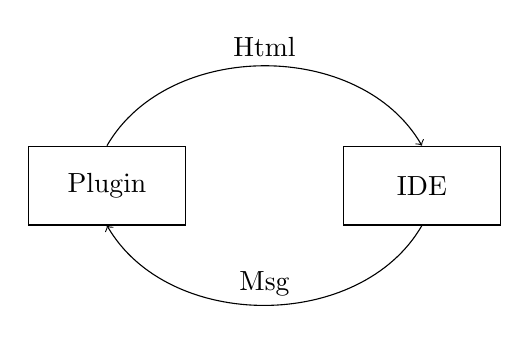
\begin{tikzpicture}
  % Nodes
  \node (p) [rectangle, draw, minimum height=1cm, minimum width=2cm] at (0, 0) {Plugin};
  \node (i) [rectangle, draw, minimum height=1cm, minimum width=2cm] at (4, 0) {IDE};
  % Arrow
  \draw[->] (p.north) to[out=60, in=120] node[midway, above] {Html} (i.north);
  \draw[->] (i.south) to[out=-120, in=-60] node[midway, above] {Msg} (p.south);
  % Header
\end{tikzpicture}


  \caption{Module Architecture}
\end{figure}

To achieve this, a module would expose three methods, to be invoked by the core
application.

\paragraph{Init} Returns a collection of key-value-pairs, which represent
the state of the core.

\paragraph{Update} Returns a collection of key-value-pairs, which
overwrite existing key-value-pairs in the state, or are appended to the state.
Invoked every time a \textit{Msg} is sent.

\paragraph{View} Returns a collection which represents \gls{html},
which is rendered by the core.

This enables \textit{pureness}, if a module is pure, the whole application is
easier to reason about.

With this setup, however, the state is appending/overwriting -only, which means
the state can only grow.

This setup is also not really modular, as a single module cannot invoke another
module, without being impure. The only way to invoke/trigger another module, is
to throw a \textit{Msg}, which would trigger an update -> view - cycle. So
a module cannot \textit{listen} for a single message, all modules are triggered
by the same \textit{Msg}, and handled accordingly.

\begin{center}
  \begin{minted}{haskell}
data Value
  = VInt Int
  | VStr String
  | VBool Bool
  | VFloat Float
  | VLst [Value]
  | VObj [(String, Value)]

newtype State = [(String, Value)]
\end{minted}

\end{center}

\begin{minted}{haskell}
data Value
  = VInt Int
  | VStr String
  | VBool Bool
  | VFloat Float
  | VLst [Value]
  | VObj [(String, Value)]

newtype Map = [(String, Value)]

data Msg = Msg
  { msg :: String
  , val :: Value
  }
\end{minted}


\begin{center}
  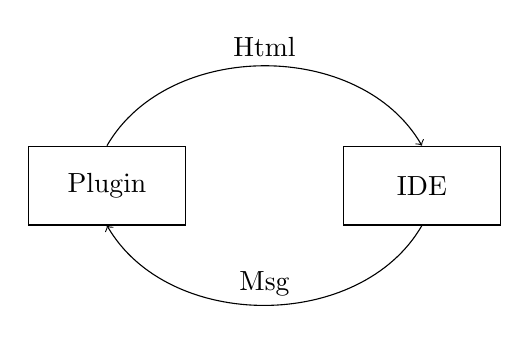
\begin{tikzpicture}
  % Nodes
  \node (p) [rectangle, draw, minimum height=1cm, minimum width=2cm] at (0, 0) {Plugin};
  \node (i) [rectangle, draw, minimum height=1cm, minimum width=2cm] at (4, 0) {IDE};
  % Arrow
  \draw[->] (p.north) to[out=60, in=120] node[midway, above] {Html} (i.north);
  \draw[->] (i.south) to[out=-120, in=-60] node[midway, above] {Msg} (p.south);
  % Header
\end{tikzpicture}


\end{center}

\subsection{State Collision}

A state collision occurs when two or more modules updates the same field, during
% NOTE: Because backend-state and frontend-state was a thing
the same update-cycle. This issue also occurs when folding two states.

% TODO: Make this less code and more text

Was \textit{solved} with this:

\begin{minted}{haskell}
  stateUpdateHandler :: [(String, Value)] -> [(String, Value)] -> [(String, TValue)]
  stateUpdateHandler fs bs = map foldPartition (group (fs ++ bs))
\end{minted}

\begin{minted}{haskell}
  foldPartition :: ([(String, Value)], [(String, [(String, Value)])]) -> ([String, [(String, Value)]]) -> (Tmap, [(String, [(String, Value)])])
  foldPartition acc cur = (map snd (head cur) : fst acc, tail cur : snd acc)
\end{minted}

Takes list of states from all plugins, checks for collisions. It returns a
list of `Either [(String, TMap)] ([(String, TMap)], String)`. If it is a
collision, then it's a `Right ([(String, TMap)], String)`, which is a tuple
where the first element is a list of tuples, being the plugin and their
state, and the last element being the field that the collision occurred on.
The other value: `Left [(String, TMap)]`, are the plugin state that has no
collision.

\paragraph{Collision} A collision between two states occurs if they share the same
field.

Example of the code in Haskell

\begin{minted}{haskell}
  stateHandler :: [(String, TMap)] -> [Either [(String, TMap)] ([(String, TMap)], String)]
  stateHandler xs = map partitionStateCollision (groupBy stateCollision xs)
  where
  -- Returns true if they have the same fields
  stateCollision :: (String, TMap) -> (String, TMap) -> Bool
  stateCollision [] _ = false
  stateCollision ((a, _):xs) ys
  | a `elem` (map fst ys) = true
  | otherwise = stateCollision xs ys
  {- Returns the collision-field
  Is only called in the context where there is a collision.
  -}
  getCollisionField :: [(String, TMap)] -> String
  getCollisionField [] = "" -- Will never happen
  getCollisionField ((a, _):ys)
  | a `elem` (map fst xs) = a
  | otherwise = getCollisionField ys
  partitionStateCollision :: [[(String, TMap)]] -> [Either [(String, TMap)] ([(String, TMap)], String)]
  partitionStateCollision [] = []
  partitionStateCollision ([ys]:xs) = Left ys : partitionStateCollision xs
  partitionStateCollision (ys:xs) =  Right (ys, getCollisionField ys) : partitionStateCollision xs
\end{minted}


There are several different ways to correct a collision between two
states:

\begin{enumerate}
  \item If the states are of same type:
    \begin{enumerate}
      \item If the value from one of the colliders are unchanged from the previous state:
        \begin{enumerate}
          \item Keep the new value OR Keep the old value
        \end{enumerate}
      \item Else
        \begin{enumerate}
          \item Apply the types' semigroup operator to the fields.
        \end{enumerate}
    \end{enumerate}
  \item Else
    \begin{enumerate}
      \item If the value from one of the colliders are unchanged from the previous state:
        \begin{enumerate}
          \item Keep the new value OR Keep the old value
        \end{enumerate}
      \item Else
        \begin{enumerate}
          \item Keep the lhs value OR Keep the rhs value
        \end{enumerate}
    \end{enumerate}
\end{enumerate}

Since the states are ordered by the name of the Plugin they come from, we
have a consistent ordering of lhs and rhs, so if the same plugins give a
collisionon the same input, given that all plugins are pure, the resulting
state will be the same every time.
The problem is that applying some function on the values could be an
unwanted way to resolve collisions. So the standard way, will be to log
the collision, and then drop both states. So even if two states have A and B
amount of fields, and just one collision, we will drop A + B amount of fields.
Therefore, for a plugin developer, they should avoid `collisions`.

\subsection{Module V.3}

Third, and hopefully the final plan:

\begin{enumerate}
    % TODO: Add footnote
  \item Everything* is a module
  \item Modules can \textit{invoke} modules
\end{enumerate}

A module only exposes a singular function:

\paragraph{Init} Returns a collection of modifications

\begin{center}
  \begin{minted}{haskell}
data Module = Module
  { name :: String
  , init :: Core -> CoreModification
  }
\end{minted}

\end{center}

\begin{center}
  \begin{minted}{haskell}
newType EventHandler = Event -> Core -> CoreModification

data Event = Event
  { moduleName :: String
  , eventName :: String
  , arguments :: Maybe Value
  }

\end{minted}

\end{center}

\begin{center}
  \begin{minted}{haskell}
module :: Module
module = Module { name = "Counter", init }

counterEvent :: Event
counterEvent = Event
  { moduleName = "CounterModule"
  , eventName = "Counter"
  , arguments = Just $ VInt 1
  }

init :: Core -> CoreModification
init core = emptyCoreModification
  { uiModification =
    [ AddUI $ Btn [Id "CounterBtn", OnClick counterEvent] [Text "Click"]
    ]
  , stateModification = [AddField "Counter" (ValInt 0)]
  , eventHandler = [("Counter", evtHdl)]
  }
\end{minted}

\end{center}

\begin{center}
  \begin{minted}{haskell}
evtHdl :: Event -> Core -> CoreModification
evtHdl evt c = case (eventName evt, arguments evt) of
  ("Counter", (Just i)) -> emptyCoreModification
    { stateModification = [UpdateField "Counter" (\x -> x + i)]
    }
  _ -> emptyCoreModification
\end{minted}

\end{center}

\subsection{Elm-Architecture}

% TODO: Insert the elm-lang architecture graph
% TODO: Also explain elm-lang

\subsection{Module Architecture}

In this application, the Elm-box is a module, while the runtime system, is the
core itself. The core invokes all modules, all of which, should have these three
functions defined:

% TODO: Add haskell code example of this

\begin{center}
  \begin{minted}{haskell}
data Value
  = VInt Int
  | VStr String
  | VBool Bool
  | VFloat Float
  | VLst [Value]
  | VObj [(String, Value)]

newtype Map = [(String, Value)]

data Msg = Msg
  { msg :: String
  , val :: Value
  }
\end{minted}

\end{center}

Firstly, the types.

% TODO: Rename `Model` to `State` or something similar
\paragraph{Model}
Model is the \textit{state} of the application. In this case, it has the same
structure as a JSON object. A few values are set at the start of the
application, so it looks like this:

% TODO: Insert some code-snippet that showcases the model
% \text{\{ "location": \{ "main": \[ \] \} \}}

% TODO: Should probably explain before-hand that the core uses webview to
% display stuff.
So, the way any module inserts \gls{html} into the IDE, is by sending a tuple,
of the \gls{html}, and Location, which is where the HTML element should be
inserted. Main corresponds to the <main>-tag in a standard \gls{html} document,
like so:

html > body > main

But this introduces a possibility for some hierarchy in the module ecosystem.
For example, a module could act as a framework, and therefore needs to only be
loaded once, creating new locations, with styling.


\paragraph{*HTML}
Just a representation of \gls{html}
% TODO: Expand


\paragraph{Location}
Just a type-alias for String, to ensure type-safety
% TODO: Expand


\paragraph{Msg}
Modules create Msg-s, that are sent to all other plugins that subscribe to them.

For example, if a module creates some Button, that when pressed sends
Msg "\textit{btn\-clicked}", then any module that are listening for this message,
can pick it up, when a user clicks on the button, and then optionally change the
Model.
